\documentclass[11pt]{article}

\usepackage[margin=1in]{geometry}
\usepackage[T1]{fontenc}
\usepackage[utf8]{inputenc}
\usepackage{lmodern}
\usepackage{microtype}
\usepackage{amsmath, amssymb, amsfonts}
\usepackage{booktabs}
\usepackage{multirow}
\usepackage{graphicx}
\usepackage{subcaption}
\usepackage{float}
\usepackage{hyperref}
\usepackage[nameinlink,noabbrev]{cleveref}
\usepackage{xcolor}
\usepackage{enumitem}

\hypersetup{
  colorlinks=true,
  linkcolor=blue!60!black,
  citecolor=blue!60!black,
  urlcolor=blue!60!black
}

\title{\textbf{DeepLOB Reproduction on FI-2010 and Transfer to Optiver Limit Order Book Data}}
\author{
Xiaoyang Xiao (Student ID: 3041882132) \\
Chun-Kai Hsu (Student ID: 3040748636) \\
Ruoyang Li (Student ID: 3041873903)
}
\date{Spring 2026}

\begin{document}
\maketitle

\begin{abstract}
We study whether a deep neural architecture originally proposed for limit order book (LOB) forecasting, DeepLOB, can be reproduced on the FI-2010 benchmark and then transferred to a materially different market dataset from Optiver. Our project has two linked goals. First, we reproduce the core CNN--Inception--LSTM pipeline on FI-2010 and verify that it achieves strong mid-price direction classification performance across multiple event horizons. Second, we adapt the architecture to Optiver's two-level book representation, introduce causal normalization and transfer-learning protocols, and evaluate zero-shot generalization, per-stock fine-tuning, and same-stock out-of-sample training. On FI-2010, the reproduced model reaches its strongest performance at longer horizons, with accuracy rising from $0.766$ at 10 events to roughly $0.795$ at 100 events and Matthews correlation coefficient (MCC) rising from $0.426$ to $0.692$. We further analyze engineered microstructure factors, show that price/volume derivative features are consistently predictive, and confirm that DeepLOB outperforms shallow manual-factor baselines. On Optiver, however, transfer is much harder: a universal model produces limited zero-shot generalization, and fine-tuning improves agreement metrics more than raw accuracy, revealing a substantial domain-shift problem rather than a simple optimization issue. The resulting report presents both positive and negative findings: DeepLOB is reproducible on FI-2010, but naive transfer to Optiver is unstable and motivates dataset-specific modeling changes.
\end{abstract}

\section{Problem Definition}
This project asks two connected technical questions:
\begin{enumerate}[leftmargin=*]
    \item Can we faithfully reproduce the main empirical behavior of DeepLOB on the FI-2010 benchmark using a modern PyTorch implementation?
    \item If so, how well does the same modeling idea transfer to a different LOB environment, namely Optiver's two-level auction book data, after architectural adaptation and fine-tuning?
\end{enumerate}

These questions are worth studying for two reasons. First, LOB prediction is a canonical sequential learning problem with strong local structure, temporal dependence, and severe class imbalance, making it a natural testbed for course ideas in representation learning and generalization. Second, successful performance on a benchmark does not guarantee transfer to a new market or data schema. Understanding where transfer succeeds and fails is practically important and scientifically useful.

Our final deliverable is therefore not just a reproduction. It is a controlled study of how far the DeepLOB design carries beyond FI-2010, and what breaks when the data distribution, label process, and book structure change.

\section{Connection to Course Content}
This project is grounded in several topics from CS 289:
\begin{itemize}[leftmargin=*]
    \item \textbf{Supervised learning and empirical risk minimization.} Both FI-2010 and Optiver tasks are formulated as multi-class classification of future mid-price direction from recent LOB states.
    \item \textbf{Deep sequence models.} The model combines convolutional feature extraction with recurrent temporal aggregation, illustrating how inductive bias matters for structured time series.
    \item \textbf{Optimization and regularization.} We use Adam, weight decay, dropout, early stopping, gradient clipping, and label smoothing, and we explicitly study how optimizer choices affect stability.
    \item \textbf{Class imbalance and evaluation.} Accuracy alone is misleading for LOB data, so we track macro-F1, Cohen's $\kappa$, and MCC. This directly reflects course discussions about metric choice under skewed labels.
    \item \textbf{Transfer learning and distribution shift.} The Optiver portion tests zero-shot transfer, head-only versus deeper fine-tuning, and stock-level heterogeneity.
    \item \textbf{Baselines and ablations.} We compare DeepLOB against logistic regression and an MLP on engineered features, and we compare universal, fine-tuned, and stock-specific Optiver models under matched evaluation.
\end{itemize}

\section{Prior Work}
DeepLOB, introduced by Zhang, Zohren, and Roberts \cite{zhang2019deeplob}, is a well-known architecture for high-frequency LOB forecasting. Its core idea is to combine local convolutional pattern extraction, an Inception-style multi-scale module, and an LSTM that aggregates short-term temporal structure before classification. The benchmark most closely associated with this line of work is FI-2010, curated by Ntakaris et al.~\cite{ntakaris2018benchmark}, which provides a standardized setup for mid-price movement prediction across several event horizons.

Earlier work on LOB prediction often relied on handcrafted microstructure features and simpler classifiers. Kercheval and Zhang \cite{kercheval2015modelling}, for example, studied machine learning methods on LOB-derived features, highlighting that engineered factors such as imbalance and order-flow statistics can contain predictive information. This matters for our project because part of our contribution is to compare DeepLOB with manual-factor baselines instead of treating the deep model as a black box.

More broadly, financial time-series forecasting is known to be sensitive to nonstationarity, label definition, and market-specific effects. Methods that work on one dataset can degrade sharply under even moderate shifts in trading regime, tick structure, or normalization scheme. That concern motivates our Optiver study. Rather than proposing a novel architecture from scratch, we investigate whether a proven LOB model can generalize to a new setting with only modest adaptation.

\section{Data and Experimental Setup}
\subsection{FI-2010}
FI-2010 contains normalized limit order book data with 40 input features corresponding to 10 bid/ask levels and associated volumes. Following the standard setup, the task is three-class classification of future mid-price movement at five event horizons: 10, 20, 30, 50, and 100 events ahead. In the codebase, these appear as horizon indices $k \in \{0,\dots,4\}$.

The training pipeline uses a lookback window of 100 events. The repository splits the provided training set into train and validation partitions and evaluates on the concatenated benchmark test files. Although the final report focus is the retained $k=3,4,5$ slice (30, 50, and 100 events), the active results directory contains the full five-horizon evaluation, which we summarize for completeness.

\subsection{Optiver}
The Optiver dataset is substantially different. Each event contains only two order book levels, yielding 8 raw LOB features after reordering:
\[
\{\texttt{ask\_price1}, \texttt{ask\_size1}, \texttt{bid\_price1}, \texttt{bid\_size1},
\texttt{ask\_price2}, \texttt{ask\_size2}, \texttt{bid\_price2}, \texttt{bid\_size2}\}.
\]

Labels are built from future mid-price returns, and preprocessing applies \emph{causal} normalization so that each event is standardized only from past information. This is an important design choice: it avoids lookahead leakage that would otherwise be easy to introduce in event-wise normalization.

The retained Optiver report slice focuses on the 5-event horizon. The saved artifacts evaluate five held-out transfer stocks, and the corresponding result files in the repository are for stock IDs 90, 99, 108, 116, and 126. For this retained slice, the preprocessing and training scripts operate on per-stock \texttt{.npz} files, which makes the experimental design explicit: each stock can be evaluated under zero-shot transfer, per-stock fine-tuning, and stock-specific temporal generalization without changing the rest of the pipeline.

\subsection{Evaluation Metrics}
Across experiments we report accuracy, Cohen's $\kappa$, MCC, and class-wise or weighted F1 scores. For Optiver we also compare regime-style profit proxies included by the project scripts, but we treat those as secondary diagnostic metrics rather than direct evidence of a deployable trading strategy.

\subsection{Retained Report Slice}
The repository contains a longer experimental history, but the cleaned final project focuses on the subset that is most coherent for a course report. Concretely:
\begin{itemize}[leftmargin=*]
    \item for FI-2010, we emphasize the 30-, 50-, and 100-event horizons;
    \item for Optiver, we emphasize the 5-event horizon and five held-out stocks;
    \item the notebook and report are therefore aligned with the saved artifacts under \texttt{results/} rather than every configuration explored during development.
\end{itemize}
This choice makes the report easier to read while still preserving the core scientific story.

\section{Approach}
\subsection{DeepLOB Reproduction on FI-2010}
Our FI-2010 model follows the DeepLOB design closely. The input tensor has shape $(B,1,T,40)$ with $T=100$. The network contains:
\begin{itemize}[leftmargin=*]
    \item three convolutional blocks that progressively merge local price-volume structure,
    \item an Inception-style multi-branch module that captures patterns at multiple receptive fields,
    \item a one-layer LSTM with hidden size 64,
    \item a dropout layer and final fully connected classifier over the three movement classes.
\end{itemize}

The implementation intentionally preserves the architectural logic of the paper while stabilizing optimization. In our environment, a literal paper-style optimizer was unreliable and often collapsed to the majority stationary class. We therefore use a tuned training profile with Adam, horizon-specific regularization, early stopping, optional class weighting, and monitor choices that differ across horizons. Shorter horizons use metrics such as macro-F1 or MCC to avoid stationary-class collapse, while longer horizons monitor validation loss.

The retained FI-2010 training configuration uses batch size 32, maximum 100 epochs, and horizon-aware regularization. For the longest horizon, which proved the most stable and most informative in the final report, the tuned configuration uses learning rate $7\times 10^{-4}$, weight decay $3\times 10^{-4}$, dropout $0.30$, label smoothing $0.02$, and gradient clipping at 1.0. These are implementation details, but they matter because the main reproduction challenge was not architectural ambiguity; it was optimization stability.

\subsection{Microstructure Analysis on FI-2010}
Beyond reproducing DeepLOB, the project includes a CPU-side analysis pipeline for engineered factors. This pipeline:
\begin{itemize}[leftmargin=*]
    \item runs Newey--West predictability tests on engineered LOB features,
    \item checks rolling-window significance stability,
    \item measures monotonicity and rank information coefficient behavior,
    \item applies Benjamini--Hochberg false discovery rate control,
    \item trains shallow baselines on manual factors,
    \item computes simple strategy-style statistics from model predictions.
\end{itemize}

This extends the project from ``does the network work?'' to ``what information seems predictive, and how much value does the deep model add over simpler alternatives?''

\subsection{DeepLOBLite for Optiver}
To transfer the method to Optiver, we adapt the network to the two-level book. The main architectural change is purely at the input interface: the model consumes $(B,1,T,8)$ instead of $(B,1,T,40)$, and the third convolutional block uses a $(1,2)$ kernel rather than the original width designed for 10 levels. The LSTM and classifier dimensions are otherwise kept the same. We refer to this adapted model as \textbf{DeepLOBLite}.

The Optiver pipeline has three stages:
\begin{enumerate}[leftmargin=*]
    \item \textbf{Universal base training:} train on a pool of source stocks and evaluate zero-shot on held-out stocks.
    \item \textbf{Transfer learning:} fine-tune the universal model separately for each held-out stock, typically updating the prediction head or a slightly deeper subset of layers.
    \item \textbf{Specific-stock out-of-sample training:} train a model on an early temporal segment of one stock and evaluate on a later segment of the same stock.
\end{enumerate}

For the retained 5-event Optiver slice, the configuration uses focal loss, dropout 0.30, weight decay, gradient clipping, macro-F1-based monitoring, and a small auxiliary regression head on future log return. The intent is to reduce majority-class collapse while preserving the original classification target.

The Optiver preprocessing pipeline is also an important part of the approach. We do not simply feed raw book values to the network. Instead, we compute mid-price based labels, apply rolling causal normalization, clip normalized features to a bounded range, and save stock-specific arrays so that each downstream experiment is reproducible and free from cross-stock preprocessing leakage.

\section{Our Contribution}
Our contribution has three distinct parts.

\subsection{Contribution 1: A Reproducible DeepLOB Pipeline with Stability Fixes}
We reimplemented the end-to-end DeepLOB workflow in a standalone training script and documented a practical issue that is easy to miss in paper reproduction: the nominal architecture is not enough if the optimizer configuration is unstable. In our environment, naive settings led to exploding validation loss and stationary-class collapse. We addressed this with horizon-aware regularization, better monitoring metrics, and safer training defaults. This is a modest but real contribution because it turns a brittle reproduction into a reliable experimental system.

\subsection{Contribution 2: Extending the FI-2010 Study Beyond Raw Benchmark Accuracy}
Instead of stopping at classification scores, we asked what the dataset itself reveals about microstructure signals. We tested 104 engineered factors, measured statistical significance with Newey--West corrections, screened them with rolling stability and false discovery rate control, and compared the deep model against manual-factor baselines. This produces a more interpretable picture of what information is present in the benchmark and how DeepLOB relates to simpler alternatives.

\subsection{Contribution 3: Transferring DeepLOB to a New Dataset and Evaluating Failure Modes}
The main original research component is the Optiver study. We adapted DeepLOB to a new LOB representation, built a causal preprocessing pipeline, and evaluated three regimes under the same retained horizon:
\begin{itemize}[leftmargin=*]
    \item universal zero-shot transfer,
    \item per-stock fine-tuning,
    \item stock-specific temporal generalization.
\end{itemize}

This is exactly the kind of modest but meaningful project extension described in the course rubric: a known method applied to a new dataset, with careful evaluation. Importantly, the result is not uniformly positive. The transfer pipeline exposes significant domain shift, and the negative result itself is a central finding of the project.

An additional contribution is that our transfer study is controlled rather than anecdotal. The universal, fine-tuned, and stock-specific models all use the same adapted architecture family and are evaluated on the same held-out stocks, which makes the comparison interpretable. That makes it possible to attribute performance gaps to transfer difficulty rather than to a hidden architectural confound.

\section{Results and Discussion}
\subsection{FI-2010 Classification Performance}
\cref{tab:fi-main} summarizes the reproduced DeepLOB results. Performance improves substantially as the prediction horizon gets longer. While 10-event prediction remains difficult and skewed toward the stationary class, the 50- and 100-event tasks produce much stronger balanced metrics.

\begin{table}[H]
\centering
\caption{DeepLOB performance on FI-2010 across benchmark event horizons.}
\label{tab:fi-main}
\begin{tabular}{lcccc}
\toprule
Horizon & Accuracy & Cohen's $\kappa$ & MCC & Weighted F1 \\
\midrule
10 events & 0.7656 & 0.3988 & 0.4255 & 0.7176 \\
20 events & 0.7487 & 0.4842 & 0.5022 & 0.7300 \\
30 events & 0.7752 & 0.6041 & 0.6076 & 0.7698 \\
50 events & 0.7972 & 0.6782 & 0.6792 & 0.7954 \\
100 events & 0.7948 & 0.6921 & 0.6923 & 0.7952 \\
\bottomrule
\end{tabular}
\end{table}

Two patterns stand out. First, MCC and $\kappa$ increase almost monotonically with horizon, suggesting that longer-horizon labels are less dominated by ambiguous stationary states. Second, the best balanced performance occurs at the 100-event horizon even though raw accuracy slightly peaks at 50 events. This is why including agreement-based metrics matters.

\begin{figure}[H]
\centering
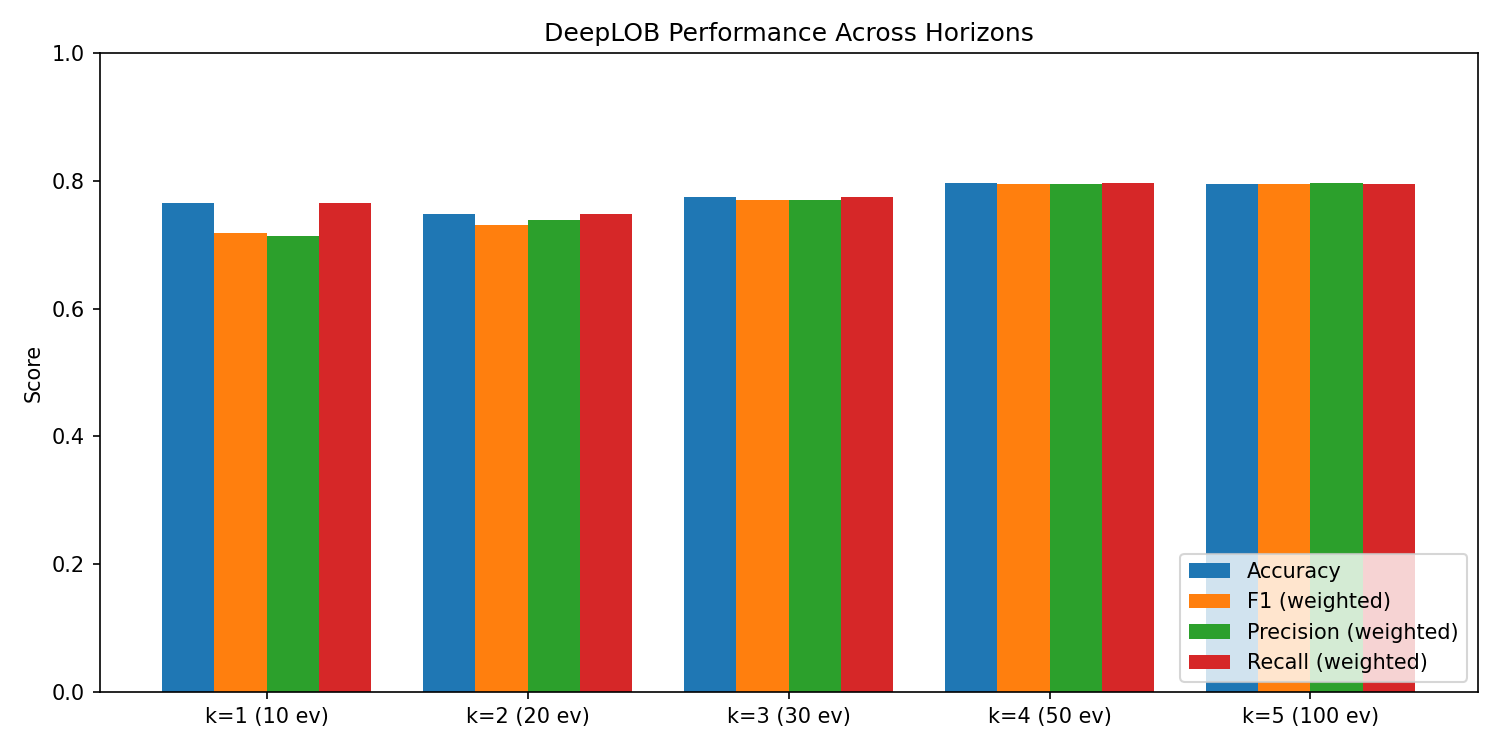
\includegraphics[width=0.78\textwidth]{../results/comparison_horizons.png}
\caption{Comparison of FI-2010 performance across horizons from the project analysis pipeline.}
\label{fig:fi-horizons}
\end{figure}

\subsection{FI-2010 Baselines and Factor Analysis}
The manual-factor baselines underperform the deep model. For the short-horizon slice included in the baseline comparison file, ridge logistic regression reaches accuracy $0.7099$ with near-zero $\kappa$, and a two-layer MLP reaches accuracy $0.7156$ with MCC $0.1908$. DeepLOB improves accuracy to $0.7656$ and MCC to $0.4255$. This gap suggests that the deep architecture is not merely matching what linear or shallow nonlinear models can already extract from a fixed factor set.

The factor analysis provides a complementary view. Out of 104 engineered features tested, 21 survive the qualification pipeline recorded in \texttt{qualified\_factors.csv}. Most of the strongest signals belong to the ``price \& volume derivatives'' group (set \texttt{u6}), and several show very large Newey--West statistics. For example, feature 1 in this group has $t_{\text{NW}}=11.29$, and feature 3 has $t_{\text{NW}}=10.84$. Rolling-window analysis also shows that many of these factors remain significant across a large fraction of windows, indicating that their predictive content is not driven by a single isolated regime.

This interpretability layer is useful for the overall project narrative. It suggests that DeepLOB is not succeeding because the benchmark is entirely inscrutable or because the network is exploiting accidental artifacts. Instead, there is evidence that the data contain stable microstructure signals, especially in derivative-style price/volume features, and the deep model appears better able to combine them over time.

\begin{figure}[H]
\centering
\begin{subfigure}[b]{0.49\textwidth}
    \centering
    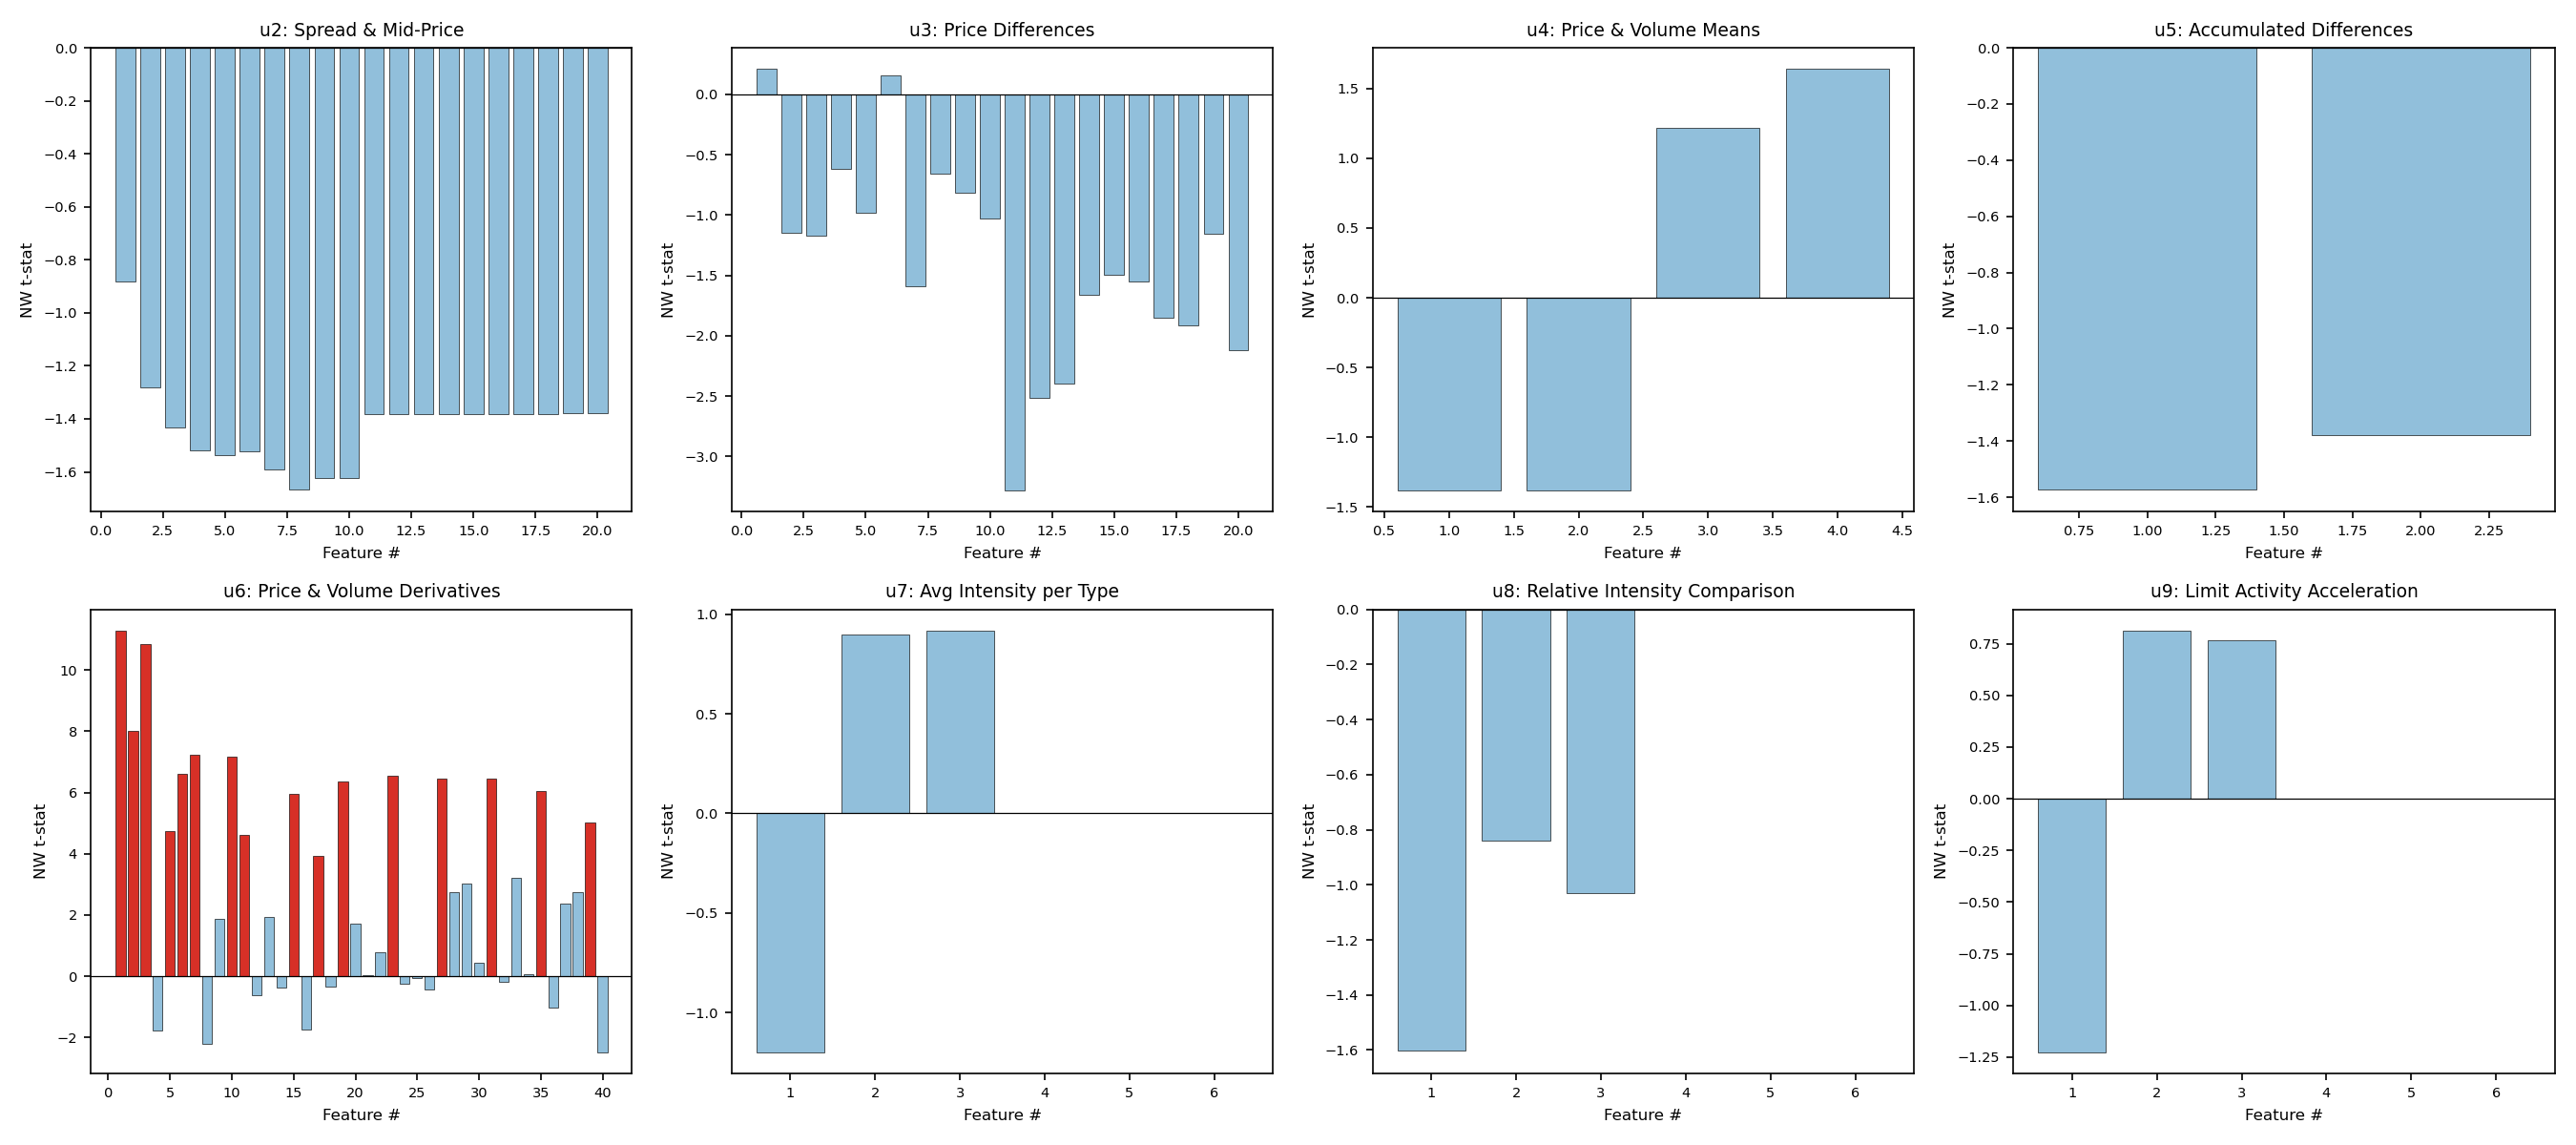
\includegraphics[width=\textwidth]{../results/feature_nw_ttest.png}
    \caption{Newey--West feature significance}
\end{subfigure}
\hfill
\begin{subfigure}[b]{0.49\textwidth}
    \centering
    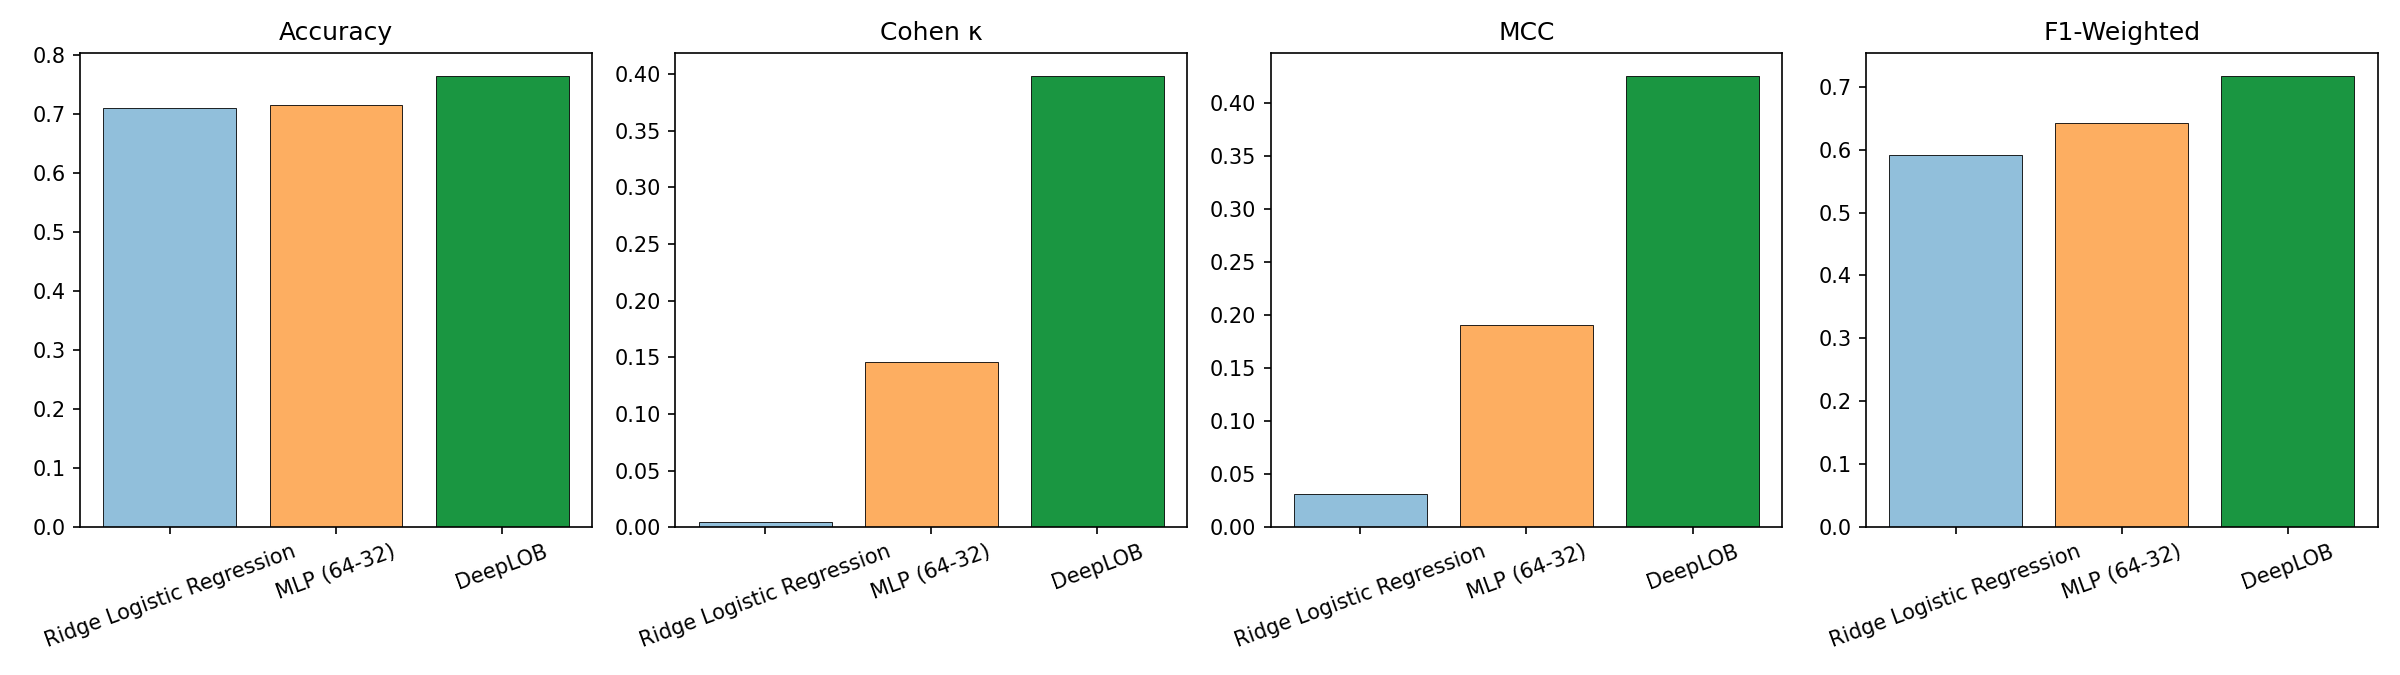
\includegraphics[width=\textwidth]{../results/baseline_comparison.png}
    \caption{Baseline model comparison}
\end{subfigure}
\caption{FI-2010 interpretability and baseline comparison results.}
\label{fig:fi-factors}
\end{figure}

One honest limitation is that the strategy-style pseudo-PnL diagnostics are weak. The saved \texttt{trading\_strategy\_stats.csv} file shows no statistically significant positive trading result, and the longer horizons are actually negative under the simplistic signal-to-PnL mapping. We view this as expected rather than disappointing: classification improvement on a benchmark does not automatically imply profitable trading once action mapping and market frictions are considered.

\subsection{Optiver Transfer Results}
The Optiver results are the most informative part of the project because they reveal where transfer fails. For the retained 5-event slice, the mean zero-shot accuracy of the universal model across the five held-out stocks is $0.3782$, with essentially zero average $\kappa$ ($0.0005$). This already suggests that the model has limited cross-stock generalization.

Fine-tuning does not improve raw accuracy on average. In fact, the mean accuracy drops from $0.3804$ to $0.2284$ across the five transfer-study stocks. However, average $\kappa$ increases from $0.0007$ to $0.0146$. That combination is unusual but meaningful: fine-tuning appears to move the model away from a trivial dominant-class predictor, yet the resulting predictions still do not align well enough with the true label distribution to improve accuracy. In other words, the problem is not just underfitting; it is label mismatch and distribution shift.

Training a stock-specific model from scratch on an earlier temporal segment performs somewhat better than fine-tuning on average, with mean accuracy $0.3509$ and mean $\kappa$ $0.0216$, but it still falls far short of the FI-2010 benchmark behavior.

\begin{table}[H]
\centering
\caption{Optiver 5-event horizon comparison across evaluation regimes.}
\label{tab:optiver-main}
\begin{tabular}{lccc}
\toprule
Regime & Mean Accuracy & Mean Cohen's $\kappa$ & Mean MCC \\
\midrule
Universal zero-shot & 0.3782 & 0.0005 & 0.0047 \\
Per-stock fine-tuned & 0.2284 & 0.0146 & -- \\
Specific-stock OOS & 0.3509 & 0.0216 & 0.0222 \\
\bottomrule
\end{tabular}
\end{table}

\begin{figure}[H]
\centering
\begin{subfigure}[b]{0.49\textwidth}
    \centering
    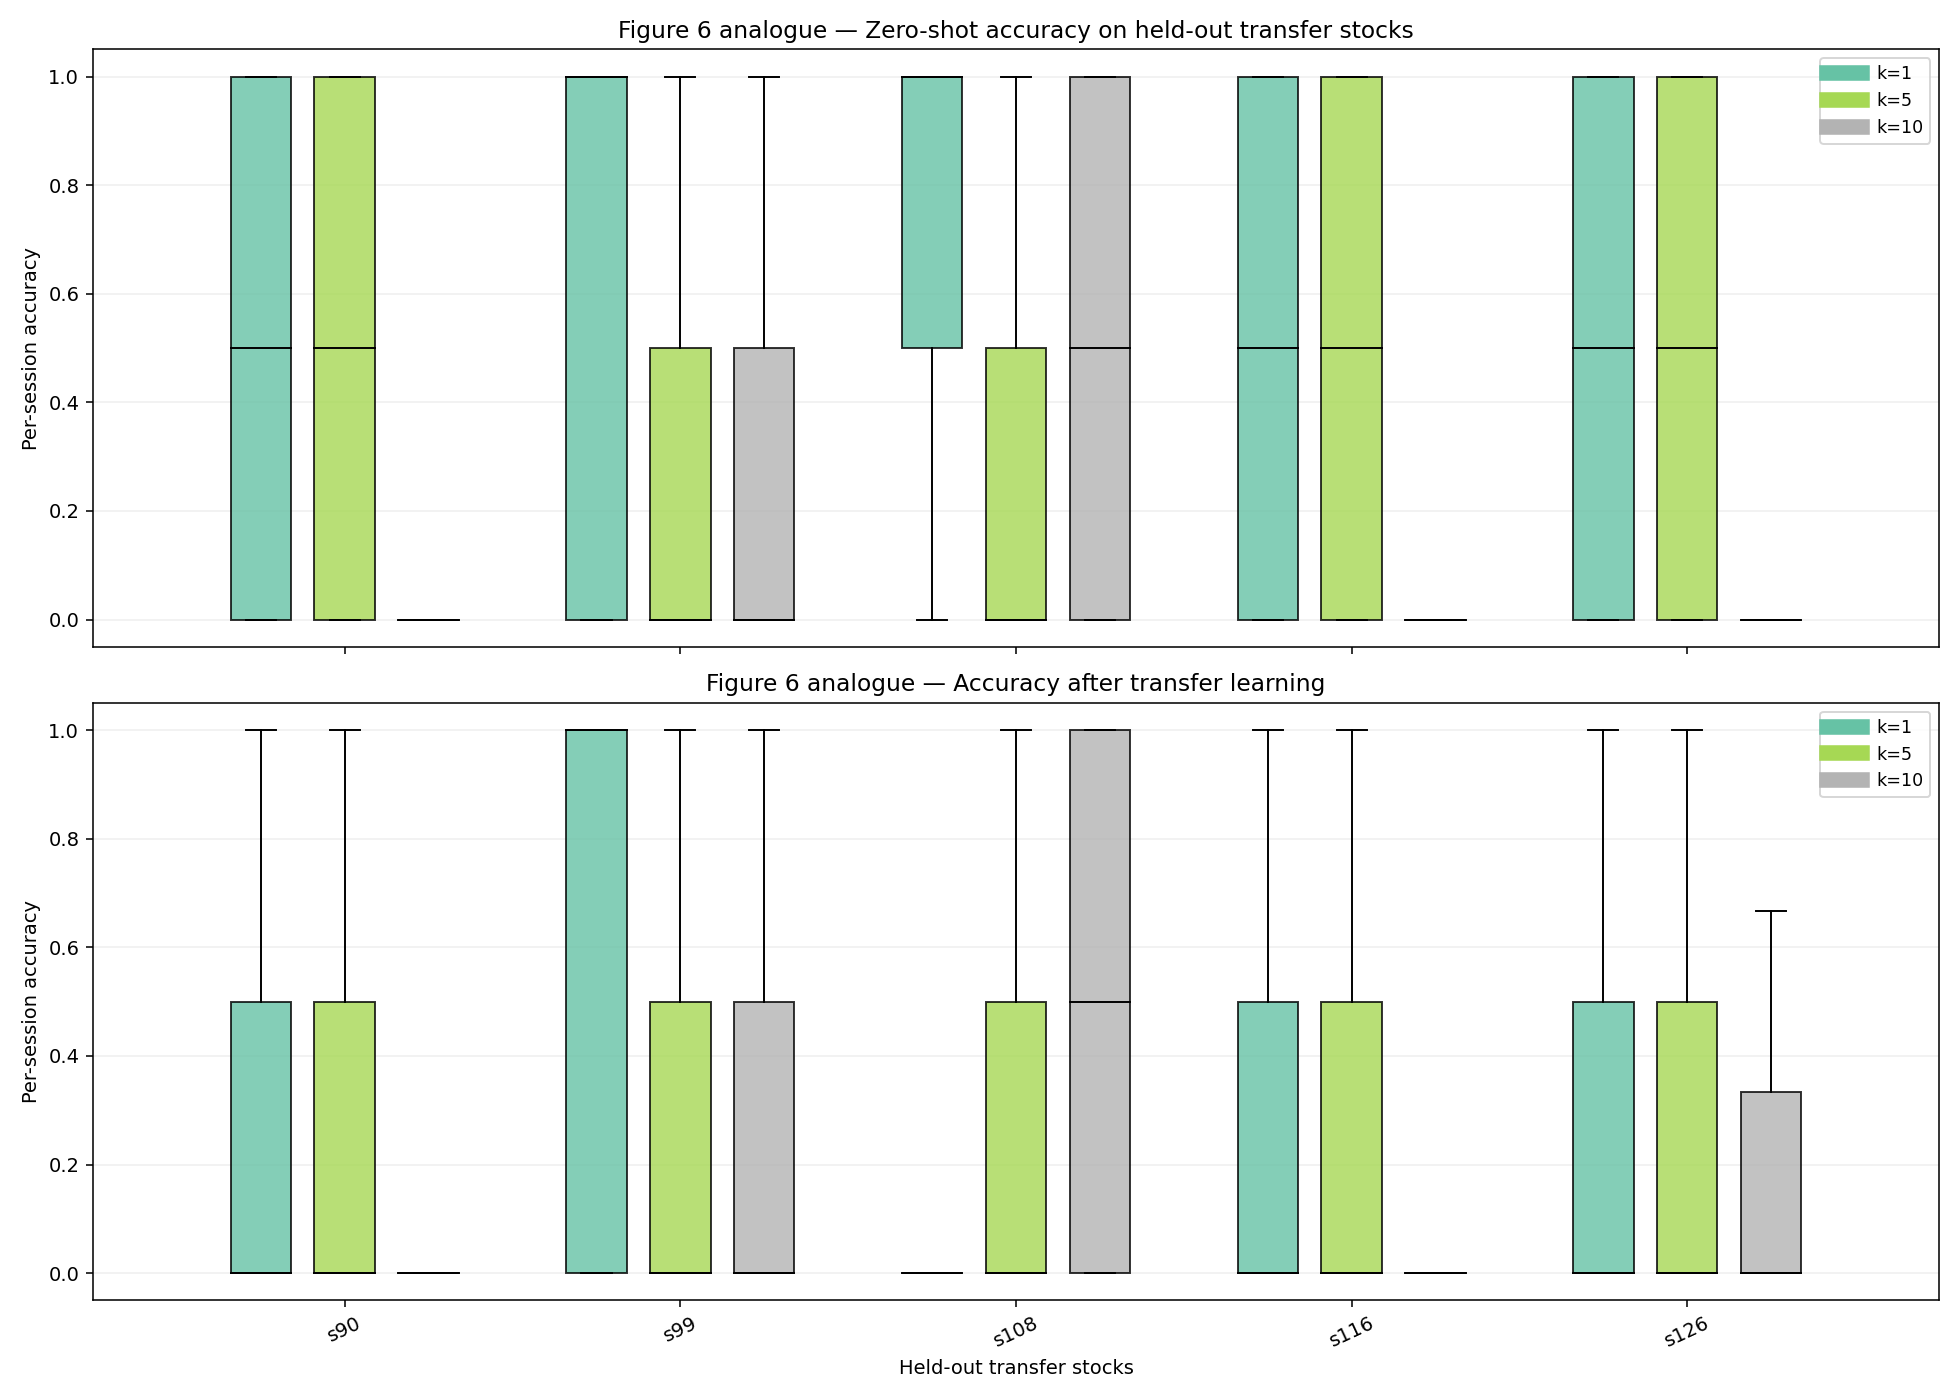
\includegraphics[width=\textwidth]{../results/optiver/figure6_transfer_accuracy.png}
    \caption{Accuracy before and after transfer}
\end{subfigure}
\hfill
\begin{subfigure}[b]{0.49\textwidth}
    \centering
    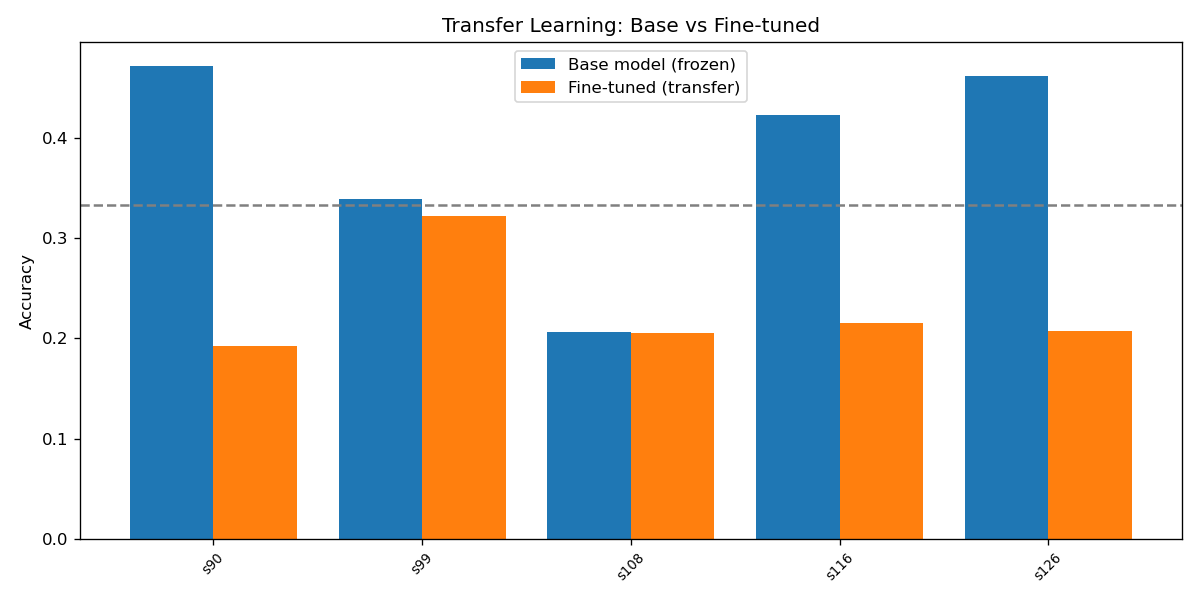
\includegraphics[width=\textwidth]{../results/optiver/transfer_comparison_k5.png}
    \caption{Universal vs transfer vs stock-specific}
\end{subfigure}
\caption{Optiver transfer-learning comparison for the retained 5-event study.}
\label{fig:optiver-transfer}
\end{figure}

\subsection{Why Did Transfer Perform Poorly?}
We believe the weak Optiver transfer performance has several causes.
\begin{itemize}[leftmargin=*]
    \item \textbf{Representation mismatch.} FI-2010 uses 10 levels while Optiver exposes only 2. Even after architectural adaptation, the available depth of queue information is dramatically smaller.
    \item \textbf{Label mismatch.} The target is still future direction classification, but the return distribution and thresholding behavior differ by stock and by dataset.
    \item \textbf{Cross-stock heterogeneity.} The held-out Optiver stocks do not appear to share one stable decision boundary. A universal model often collapses to one dominant class, and fine-tuning can over-correct into another dominant class.
    \item \textbf{Temporal nonstationarity.} Same-stock out-of-sample training performs only slightly better, suggesting that within-stock time drift is also substantial.
\end{itemize}

This negative result is important. It shows that a benchmark-winning LOB architecture is not plug-and-play across datasets, even when the task description sounds similar.

\begin{table}[H]
\centering
\caption{Per-stock Optiver accuracy for the retained 5-event horizon.}
\label{tab:optiver-per-stock}
\begin{tabular}{lccc}
\toprule
Stock ID & Zero-shot & Fine-tuned & Specific-stock OOS \\
\midrule
90  & 0.4457 & 0.1922 & 0.4083 \\
99  & 0.3348 & 0.3222 & 0.3422 \\
108 & 0.2222 & 0.2056 & 0.2033 \\
116 & 0.4313 & 0.2150 & 0.3683 \\
126 & 0.4570 & 0.2072 & 0.4322 \\
\bottomrule
\end{tabular}
\end{table}

The per-stock table makes the heterogeneity especially clear. Stocks 90, 116, and 126 have moderately decent zero-shot accuracy, but fine-tuning degrades them sharply. Stock 99 changes only slightly, while stock 108 is difficult under every regime. This dispersion suggests that there is no single ``typical'' transfer behavior, which strengthens our conclusion that stock-specific distribution shift is a first-order issue.

\section{Code and Reproducibility}
The codebase is organized to separate heavy computation from presentation:
\begin{itemize}[leftmargin=*]
    \item \texttt{scripts/train\_deeplob.py} trains DeepLOB on FI-2010.
    \item \texttt{scripts/analyze\_fi2010.py} produces feature tests, baselines, and trading-style diagnostics.
    \item \texttt{scripts/prepare\_optiver.py} preprocesses Optiver data with causal normalization.
    \item \texttt{scripts/train\_optiver.py} runs universal training, transfer learning, and stock-specific evaluation.
    \item \texttt{scripts/analyze\_optiver.py} builds notebook-ready summary figures.
    \item the top-level notebooks load saved artifacts and present the experiments in report form.
\end{itemize}

This structure supports reproducibility because the expensive stages are scripted, parameterized, and saved to disk, while the notebooks act as a readable front end rather than hiding the main logic.

In addition, the repository stores trained models, result summaries, and figure artifacts in separate directories, which made it possible for our team to divide responsibilities cleanly: model development and experiment execution could proceed independently from final report writing. That workflow is particularly helpful for a course project because it lets the written report stay tightly coupled to saved outputs rather than to fragile interactive notebook state.

\section{Limitations and Future Work}
Our project has several limitations. First, although the FI-2010 reproduction is strong, the benchmark itself is relatively standardized and may not fully reflect the heterogeneity of real trading environments. Good benchmark performance therefore should not be interpreted as evidence of universal market generalization. Second, the retained Optiver study is intentionally narrow: we focus on a single final report horizon and a small set of held-out stocks so that the experiments remain interpretable and feasible within the scope of a course project. This makes the story cleaner, but it also means our conclusions about transfer should be understood as carefully measured case-study evidence rather than a comprehensive cross-market claim.

There are also modeling limitations. Our Optiver adaptation keeps the original DeepLOB inductive bias as much as possible, which is useful for controlled comparison, but it may not be the architecture best matched to a two-level order book. Likewise, while our fine-tuning experiments reveal domain shift, they do not fully isolate whether the dominant issue is feature mismatch, label construction, temporal nonstationarity, or insufficient stock-specific data. Finally, our trading-style evaluation is deliberately simple and omits realistic execution frictions, so it should be read only as a diagnostic rather than as a claim about profitability.

These limitations point naturally to future work. One direction is a more systematic Optiver ablation study comparing normalization modes, label definitions, transfer modes, and class-balancing strategies under a fixed evaluation protocol. A second direction is architectural: for example, replacing or augmenting the recurrent component with temporal convolution or attention-based sequence modeling better suited to shallow books. A third direction is broader transfer evaluation across more stocks and horizons, including calibration analysis and robustness checks under changing volatility regimes. Taken together, these extensions would help separate which parts of DeepLOB are genuinely portable from which parts are benchmark-specific.

\section{Conclusion}
This project reproduced DeepLOB successfully on FI-2010 and showed that the model's strongest benchmark performance occurs at medium-to-long horizons. We also extended the benchmark study with statistically grounded factor analysis and shallow baselines, finding that manual microstructure features contain real signal but still underperform the deep architecture.

Our main original contribution was transferring the method to Optiver. That experiment surfaced a more nuanced conclusion than a simple success story: the architecture transfers imperfectly, stock heterogeneity is strong, and fine-tuning can improve agreement metrics without improving accuracy. The project therefore demonstrates both the strength of DeepLOB as a benchmark model and the limits of benchmark-to-real-dataset generalization.

\section*{Project Summary}
In one sentence, this project:
\begin{quote}
reproduced a canonical deep LOB predictor on FI-2010, analyzed what signals drive performance, and tested how far the same idea transfers to Optiver through causal preprocessing, model adaptation, and transfer-learning experiments.
\end{quote}

\bibliographystyle{plain}
\bibliography{references}

\end{document}
